\chapter{Dynamics in Non-Inertial Reference Frames}
\label{ch:noninertial_text}

\begin{chapterintro}
\textbf{Chapter Objectives:} When studying phenomena on the rotating Earth or in accelerating vehicles, we observe from non-inertial frames. In this chapter, you will master the fundamental equation of relative dynamics; calculate centrifugal and Coriolis fictitious forces; understand plumb line deflections and the flattening of the Earth; explain why cyclones spin counter-clockwise in the Northern hemisphere; and solve the precession of the Foucault pendulum.
\end{chapterintro}

\section{The Equation of Relative Dynamics}

In an inertial frame $\mathcal{R}$, Newton's second law is strictly valid: $m\vec{a}_a = \sum\vec{F}_{\text{real}}$.
Substituting the kinematic composition of accelerations $\vec{a}_a = \vec{a}_r + \vec{a}_e + \vec{a}_c$:
\[
m\left(\vec{a}_r + \vec{a}_e + \vec{a}_c\right) = \sum\vec{F}_{\text{real}}.
\]
Rearranging to isolate the relative acceleration $\vec{a}_r$ as seen by the moving observer:
\[
\boxed{m\vec{a}_r = \sum\vec{F}_{\text{real}} + \vec{F}_{ie} + \vec{F}_{ic}}
\]
where the two \textbf{fictitious (inertial) forces} are:
\begin{align}
\vec{F}_{ie} &= -m\vec{a}_e \quad \text{(\textbf{Inertial Force of Transport / Centrifugal Force})}, \\
\vec{F}_{ic} &= -m\vec{a}_c = -2m\,\vec{\Omega}\times\vec{v}_r \quad \text{(\textbf{Coriolis Force})}.
\end{align}

\begin{historicalbox}{Léon Foucault and the Panthéon Demonstration (1851)}
\begin{minipage}{0.30\textwidth}
\centering
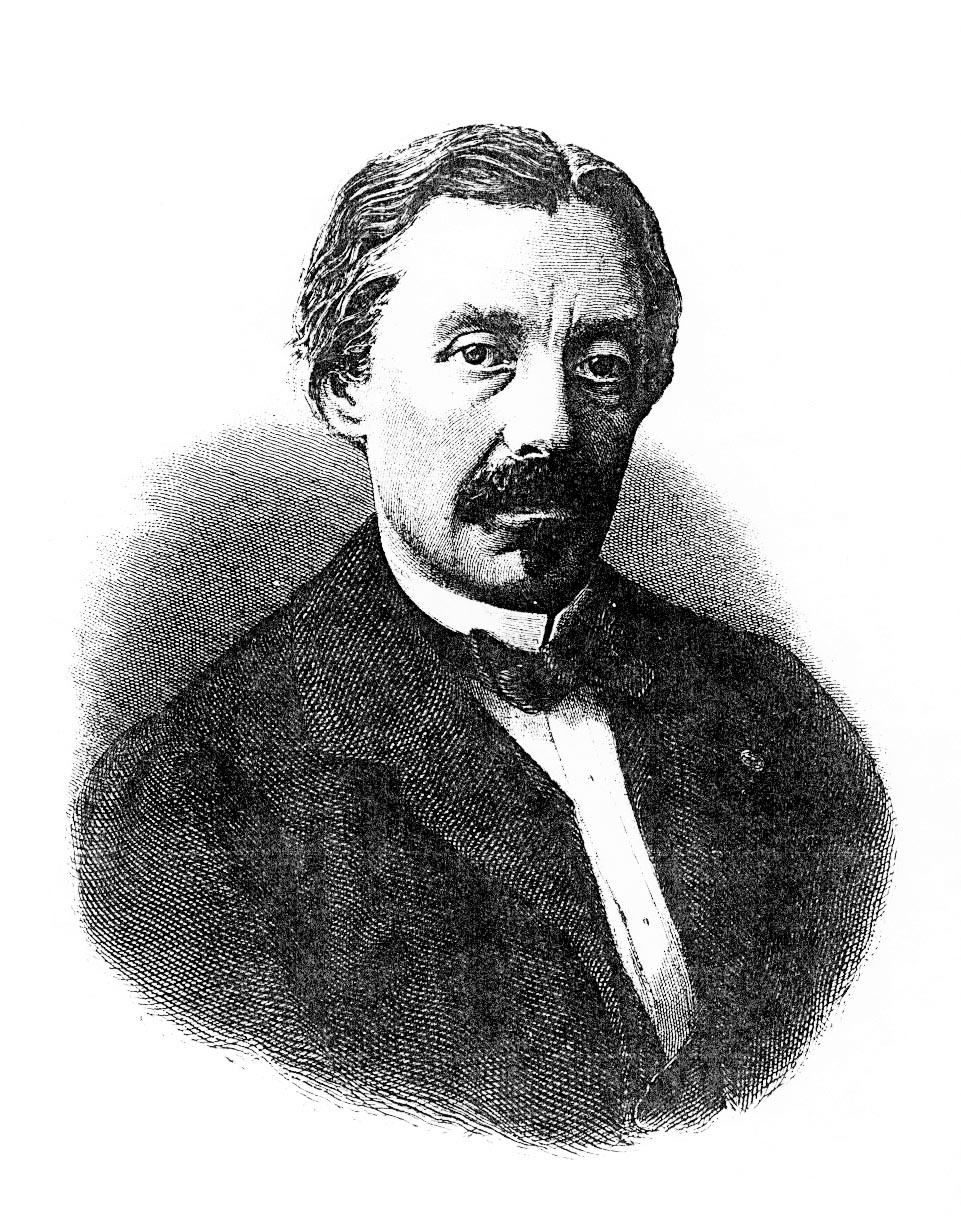
\includegraphics[width=0.92\textwidth]{images/foucault.jpg}
\vspace{4pt}
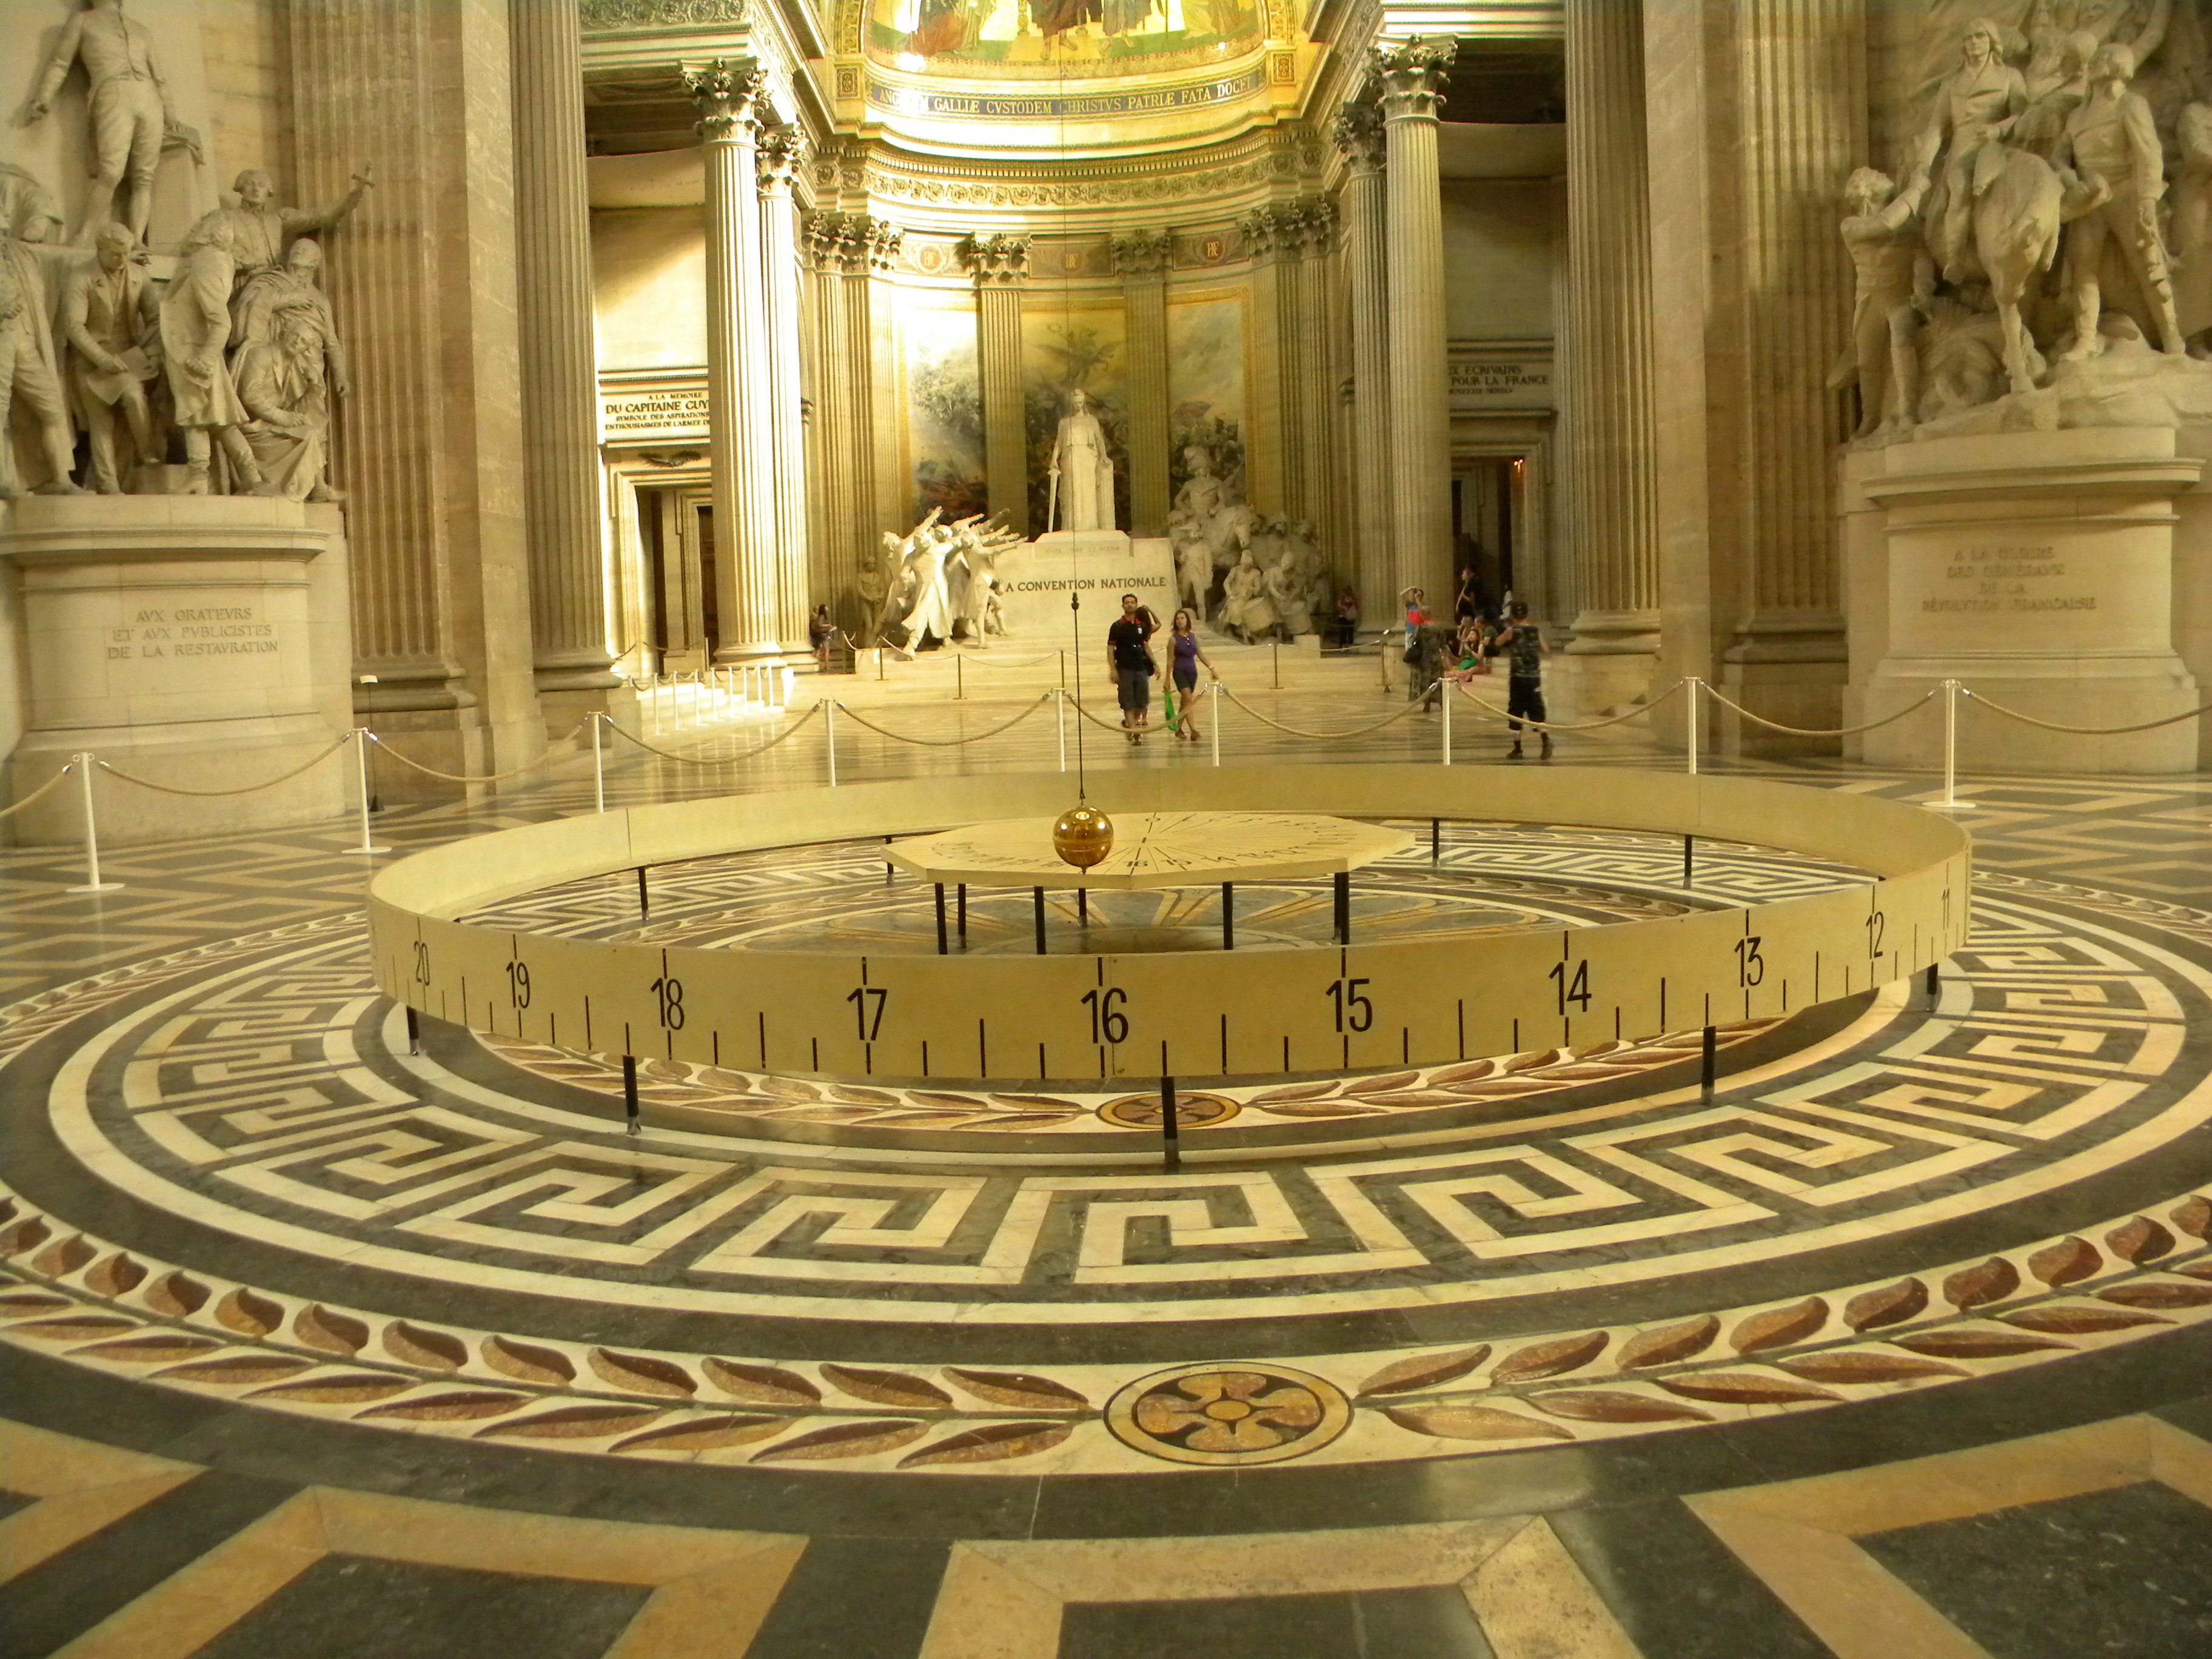
\includegraphics[width=0.92\textwidth]{images/foucault_pendulum.jpg}
\captionof{figure}{Léon Foucault (1819--1868), and the Foucault Pendulum suspended beneath the dome of the Panthéon in Paris.}
\end{minipage}\hfill
\begin{minipage}{0.66\textwidth}
In January 1851, French physicist Léon Foucault suspended a $28\ \mathrm{kg}$ brass-coated lead sphere from a $67\ \mathrm{m}$ steel wire inside the dome of the Panthéon in Paris. A spike on the bob traced lines in sand spread on the floor.

Before a mesmerized crowd, the plane of swing visibly rotated clockwise at roughly $11^\circ$ per hour, taking $31.8$ hours for a complete revolution. Foucault had devised the first purely dynamic, laboratory-based proof of Earth's rotation that did not require celestial observations: ``You are invited to see the Earth turn.''
\end{minipage}
\end{historicalbox}

\section{Centrifugal Force and Apparent Terrestrial Weight}

On the rotating Earth ($\vec{\Omega} = \Omega\khat$ with $\Omega \approx 7.292\times 10^{-5}\ \mathrm{rad\,s^{-1}}$), a body at rest relative to the surface ($\vec{v}_r = \vzero$) experiences zero Coriolis force.
However, it experiences the outward \textbf{centrifugal force}:
\[
\vec{F}_{\text{cf}} = -m\vec{\Omega}\times(\vec{\Omega}\times\vec{r}) = m\Omega^2 r_\perp\,\ur = m\Omega^2 R_E\cos\lambda\,\ur,
\]
where $\lambda$ is latitude and $r_\perp = R_E\cos\lambda$ is the distance to the polar axis.
The measured \textbf{apparent weight} is the resultant of true gravitational attraction and the centrifugal force:
\[
\boxed{\vec{P}_{\text{app}} = m\vec{g}_{\text{eff}} = m\vec{g}_0 + \vec{F}_{\text{cf}}.}
\]
\begin{itemize}[leftmargin=1.4em,itemsep=2pt]
  \item At the poles ($\lambda = \pm 90^\circ$): $r_\perp = 0 \implies \vec{F}_{\text{cf}} = \vzero$. Apparent gravity equals true gravity ($g_{\text{eff}} \approx 9.832\ \mathrm{m\,s^{-2}}$).
  \item At the equator ($\lambda = 0^\circ$): $\vec{F}_{\text{cf}}$ points directly opposite to gravity, reducing apparent weight by $\Omega^2 R_E \approx 0.034\ \mathrm{m\,s^{-2}}$ ($g_{\text{eff}} \approx 9.780\ \mathrm{m\,s^{-2}}$).
  \item At intermediate latitudes: $\vec{g}_{\text{eff}}$ is tilted slightly toward the equator, deflecting a hanging plumb line by up to $\theta \approx 6\ \text{arcminutes}$ from the true geometric center of Earth.
\end{itemize}

\section{Meteorological Consequences of the Coriolis Force}

\begin{figure}[htbp]
\centering
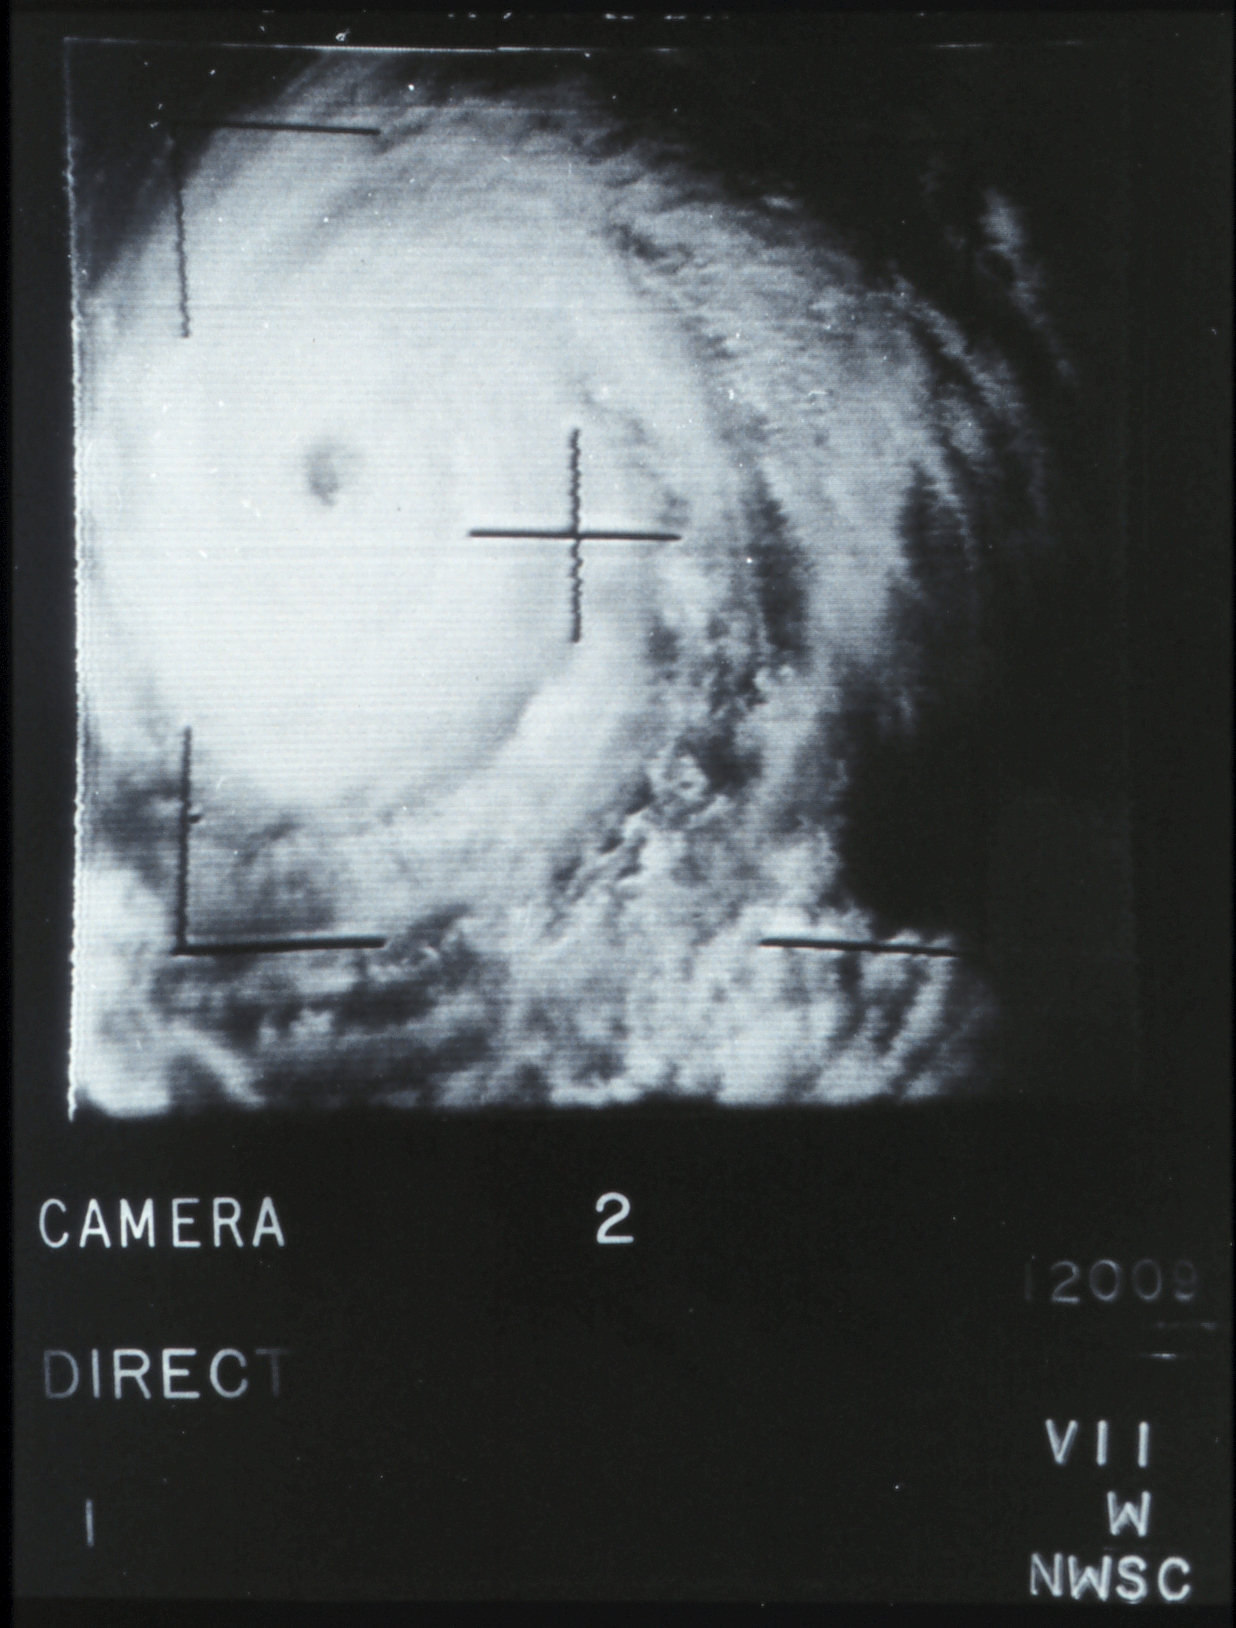
\includegraphics[width=0.62\textwidth]{images/cyclone_coriolis.jpg}
\caption{Early satellite photograph of a tropical cyclone displaying the classic counter-clockwise spiral in the Northern Hemisphere induced by the Coriolis deflection of inward-flowing air masses.}
\label{fig:cyclone}
\end{figure}

In the Northern hemisphere, Earth's angular velocity vector has an upward vertical component $\Omega_z = \Omega\sin\lambda > 0$.
The horizontal Coriolis force acting on horizontal air velocity $\vec{v}_r$ is:
\[
\vec{F}_{\text{Cor, horiz}} = -2m(\Omega\sin\lambda\khat)\times\vec{v}_r = 2m\Omega\sin\lambda(\vec{v}_r\times\khat).
\]
\begin{lawbox}{Buys Ballot's Law of Meteorology}
In the Northern hemisphere, the Coriolis force deflects every moving body \textbf{to its right}; in the Southern hemisphere, it deflects every moving body \textbf{to its left}.
When air rushes inward toward a low-pressure center (cyclone), this rightward deflection causes the inward streams to circulate \textbf{counter-clockwise} in the North, forming hurricanes and typhoons.
\end{lawbox}

\section{Extensive Worked Examples}

\begin{workedexample}{The Parabolic Liquid Telescope Mirror}
A cylindrical container filled with a reflective liquid (such as liquid mercury or molten gallium alloy) rotates about its central vertical axis at constant angular velocity $\omega$.
(a) In the rotating frame of the liquid, set up cylindrical coordinates $(r, \theta, z)$ and show that the effective gravity is $\vec{g}_{\text{eff}} = \omega^2 r\ur - g\khat$.
(b) Derive the equation of the free surface $z(r) = z_0 + \frac{\omega^2 r^2}{2g}$.
(c) Show that this surface forms a perfect parabolic mirror with focal length $f = \frac{g}{2\omega^2}$.
(d) For an astronomical telescope with focal length $f = 6.00\ \mathrm{m}$, compute the required rotation rate $\omega$ and rotational period in rpm.

\paragraph{Solution.}

(a) In the rotating frame $\mathcal{R}'$, the fluid is at rest ($\vec{v}_r = \vzero$, $\vec{F}_{\text{Cor}} = \vzero$).
The forces acting on a fluid element of mass $\dd m = \rho\,\dd V$ are:
\begin{itemize}[leftmargin=1.4em,itemsep=2pt]
  \item True gravity: $\dd\vec{P} = -(\dd m)g\khat$.
  \item Centrifugal force: $\dd\vec{F}_{\text{cf}} = +(\dd m)\omega^2 r\,\ur$.
\end{itemize}
The effective acceleration of gravity in $\mathcal{R}'$ is:
\[
\boxed{\vec{g}_{\text{eff}} = \frac{\dd\vec{P} + \dd\vec{F}_{\text{cf}}}{\dd m} = \omega^2 r\,\ur - g\khat.}
\]

(b) At hydrostatic equilibrium in $\mathcal{R}'$, the fluid pressure gradient satisfies $\vec{\nabla} p = \rho\vec{g}_{\text{eff}}$.
Along the free surface open to the atmosphere, $p \equiv p_{\text{atm}} = \text{const}$, so $\dd p = \vec{\nabla} p\cdot\dd\vec{r} = 0$:
\[
\rho\vec{g}_{\text{eff}}\cdot\dd\vec{r} = 0 \implies \vec{g}_{\text{eff}}\perp\dd\vec{r}.
\]
In cylindrical coordinates, $\dd\vec{r} = \dd r\,\ur + r\dd\theta\,\ut + \dd z\,\khat$:
\[
(\omega^2 r\,\ur - g\khat)\cdot(\dd r\,\ur + \dd z\,\khat) = 0 \implies \omega^2 r\,\dd r - g\,\dd z = 0.
\]
Separating variables:
\[
\dd z = \frac{\omega^2}{g}r\,\dd r.
\]
Integrating with $z(0) = z_0$:
\[
\boxed{z(r) = z_0 + \frac{\omega^2 r^2}{2g}.}
\]
The free surface is an exact \textbf{paraboloid of revolution}!

(c) From classical optics, a parabolic mirror described by $z(r) = \frac{r^2}{4f}$ focuses all incoming parallel on-axis light rays to a single point at focal length $f$.
Comparing coefficients:
\[
\frac{1}{4f} = \frac{\omega^2}{2g} \implies \boxed{f = \frac{g}{2\omega^2}.}
\]
The focal length is determined solely by the rotation speed $\omega$ and gravity!

(d) For $f = 6.00\ \mathrm{m}$:
\[
\omega = \sqrt{\frac{g}{2f}} = \sqrt{\frac{9.81}{2(6.00)}} = \sqrt{\frac{9.81}{12.0}} = \sqrt{0.8175} \approx \mathbf{0.904\ \mathrm{rad\,s^{-1}}.}
\]
Rotational speed in revolutions per minute:
\[
N = \frac{\omega\times 60}{2\pi} = \frac{0.904\times 60}{2\pi} \approx \mathbf{8.63\ \mathrm{rpm}.}
\]
A gentle rotation of under $9$ rpm creates a giant $6$-meter focal length optical mirror for astronomical observatories at a fraction of the cost of polishing glass!
\end{workedexample}

\begin{workedexample}{Analytical Solution of the Foucault Pendulum}
A simple pendulum of length $L$ and bob mass $m$ is suspended at latitude $\lambda$. For small horizontal oscillations ($z \approx 0$), the string tension is $T \approx mg$.
(a) Write the horizontal equations of motion in the rotating Earth frame:
\begin{align*}
\ddot{x} - 2\omega_z\dot{y} + \omega_0^2 x &= 0, \\
\ddot{y} + 2\omega_z\dot{x} + \omega_0^2 y &= 0,
\end{align*}
where $\omega_0 = \sqrt{g/L}$ and $\omega_z = \Omega\sin\lambda$.
(b) Introduce the complex coordinate $\zeta(t) = x(t) + \mathrm{i}y(t)$ and solve for $\zeta(t)$ with initial release $\zeta(0) = x_0, \dot{\zeta}(0) = 0$.
(c) Prove that the plane of oscillation rotates with angular velocity $\Omega_F = -\Omega\sin\lambda$.

\paragraph{Solution.}

(a) Set up local axes: $x$ pointing East, $y$ pointing North, $z$ pointing vertically upward (Zenith).
Earth's rotation vector is $\vec{\Omega} = \Omega\cos\lambda\jhat + \Omega\sin\lambda\khat$.
For small oscillations, the restoring force from the string has horizontal components:
\[
F_{x,\text{rest}} \approx -mg\frac{x}{L} = -m\omega_0^2 x, \qquad F_{y,\text{rest}} \approx -mg\frac{y}{L} = -m\omega_0^2 y.
\]
The Coriolis force on horizontal velocity $\vec{v}_r = \dot{x}\ihat + \dot{y}\jhat$ is:
\[
\vec{F}_{\text{Cor}} = -2m\vec{\Omega}\times\vec{v}_r = -2m\begin{vmatrix} \ihat & \jhat & \khat \\ 0 & \Omega\cos\lambda & \Omega\sin\lambda \\ \dot{x} & \dot{y} & 0 \end{vmatrix} = 2m(\Omega\sin\lambda\dot{y})\ihat - 2m(\Omega\sin\lambda\dot{x})\jhat + 2m(\Omega\cos\lambda\dot{x})\khat.
\]
Defining $\omega_z = \Omega\sin\lambda$, Newton's second law along $x$ and $y$ gives:
\begin{align*}
m\ddot{x} &= -m\omega_0^2 x + 2m\omega_z\dot{y} \implies \boxed{\ddot{x} - 2\omega_z\dot{y} + \omega_0^2 x = 0,} \\
m\ddot{y} &= -m\omega_0^2 y - 2m\omega_z\dot{x} \implies \boxed{\ddot{y} + 2\omega_z\dot{x} + \omega_0^2 y = 0.}
\end{align*}

(b) Multiply the second equation by $\mathrm{i}$ and add it to the first:
\[
(\ddot{x} + \mathrm{i}\ddot{y}) + 2\omega_z(\mathrm{i}\dot{x} - \dot{y}) + \omega_0^2(x + \mathrm{i}y) = 0.
\]
Notice that $\mathrm{i}\dot{x} - \dot{y} = \mathrm{i}(\dot{x} + \mathrm{i}\dot{y}) = \mathrm{i}\dot{\zeta}$.
Thus:
\[
\boxed{\ddot{\zeta} + 2\mathrm{i}\omega_z\dot{\zeta} + \omega_0^2\zeta = 0.}
\]
Substitute the trial solution $\zeta(t) = e^{-\mathrm{i}\omega_z t} u(t)$:
\[
\dot{\zeta} = e^{-\mathrm{i}\omega_z t}(\dot{u} - \mathrm{i}\omega_z u), \qquad \ddot{\zeta} = e^{-\mathrm{i}\omega_z t}(\ddot{u} - 2\mathrm{i}\omega_z\dot{u} - \omega_z^2 u).
\]
Substituting into the differential equation:
\[
e^{-\mathrm{i}\omega_z t}\left[ (\ddot{u} - 2\mathrm{i}\omega_z\dot{u} - \omega_z^2 u) + 2\mathrm{i}\omega_z(\dot{u} - \mathrm{i}\omega_z u) + \omega_0^2 u \right] = 0.
\]
The cross-terms cancel identically:
\[
\ddot{u} + (\omega_0^2 + \omega_z^2)u = 0.
\]
Since $\omega_z \approx 10^{-5}\ \mathrm{rad\,s^{-1}} \ll \omega_0 \approx 1\ \mathrm{rad\,s^{-1}}$, $\omega_0^2 + \omega_z^2 \approx \omega_0^2$.
The solution for $u(t)$ with $u(0) = x_0, \dot{u}(0) = 0$ is $u(t) = x_0\cos(\omega_0 t)$.
Therefore, the exact complex solution is:
\[
\boxed{\zeta(t) = x_0\cos(\omega_0 t)\,e^{-\mathrm{i}\omega_z t}.}
\]

(c) Decomposing into real and imaginary parts using Euler's formula $e^{-\mathrm{i}\omega_z t} = \cos(\omega_z t) - \mathrm{i}\sin(\omega_z t)$:
\begin{align*}
x(t) &= x_0\cos(\omega_0 t)\cos(\omega_z t), \\
y(t) &= -x_0\cos(\omega_0 t)\sin(\omega_z t).
\end{align*}
This represents rapid simple harmonic oscillations of frequency $\omega_0$ along a straight line that \textbf{rotates clockwise} with steady angular frequency:
\[
\boxed{\Omega_F = -\omega_z = -\Omega\sin\lambda.}
\]
The period of a complete $360^\circ$ rotation is:
\[
\boxed{T_F = \frac{2\pi}{\abs{\Omega_F}} = \frac{24\ \mathrm{h}}{\sin\lambda}.}
\]
At the North Pole ($\lambda = 90^\circ$), $T_F = 24.0\ \mathrm{h}$; at the Panthéon in Paris ($\lambda = 48^\circ 51'$), $T_F = \frac{24}{\sin 48.85^\circ} \approx \mathbf{31.9\ \mathrm{h}}$.
\end{workedexample}
